\documentclass[sigconf]{acmart}
\usepackage[utf8]{inputenc}
\usepackage[T1]{fontenc}
\usepackage{newtxmath}
\usepackage{graphicx}
\usepackage{amsmath}
\usepackage{algorithm}
\usepackage{algorithmic}
\usepackage{booktabs}
\usepackage{float}
\usepackage{placeins}
\usepackage{listings}
\usepackage{xcolor}
\usepackage{caption}
\usepackage{placeins} 
\usepackage{textcomp}       
\usepackage{amsmath}  
\usepackage{tabularx}
\usepackage{pgfplots}
\pgfplotsset{compat=1.18}
\usepackage{booktabs}

\FloatBarrier



\lstdefinestyle{mystyle}{
	basicstyle=\ttfamily\footnotesize,
	backgroundcolor=\color{gray!10},
	frame=single,
	keywordstyle=\color{blue},
	commentstyle=\color{green!50!black},
	breaklines=true,
	numbers=left,
	numberstyle=\tiny\color{gray},
	captionpos=b
}
\lstset{style=mystyle}

%%
%% Rights and Conference/Jmynal info (you can remove or adjust as needed)
\setcopyright{none}
\copyrightyear{2025}
\acmYear{2025}
\acmDOI{none}
\acmConference[Exam Global and Multi-Objective Optimization]{Exam Global and Multi-Objective Optimization}{2025}{Trieste, Italy}
\acmBooktitle{Exam Global and Multi-Objective Optimization}
\acmISBN{none}
\settopmatter{printacmref=false}

\title{Fantasy Football Optimization}

\author{Marco De Rito - SM3800016}
\affiliation{
	\institution{University of Trieste}
	\city{Trieste}
	\country{Italy}
}
\email{marco.derito@studenti.units.it}
\setlength{\headheight}{15.5pt}
\begin{CCSXML}
	<ccs2012>
	<concept>
	<concept_id>10002950.10003648.10003688.10003693</concept_id>
	<concept_desc>Computing methodologies~Optimization algorithms</concept_desc>
	<concept_significance>500</concept_significance>
	</concept>
	</ccs2012>
\end{CCSXML}

\ccsdesc[500]{Computing methodologies~Optimization algorithms}

\begin{document}
	\sloppy
	\begin{abstract}
		This report represents my final project for an advanced optimization course, where I develop a comprehensive methodology for fantasy football team selection, formulated as an \emph{inverse optimization problem}. I apply three well-known meta-heuristics: Particle Swarm Optimization (PSO), Differential Evolution (DE) and Evolution Strategies (ES) in a multi-manager setting, ensuring budget and positional constraints are respected.
		
		The study integrates theoretical foundations (including PSO, DE, ES, and inverse optimization principles), practical code implementations in Python (data loading, scoring, fitness function, forced assignments, multi-round auctions), and empirical evaluations. Through comparisons of budget usage, forced picks, and final team scores, I show that each algorithm delivers competitive results, albeit with differences in strategy diversity and resource utilization. Finally, I reflect on future enhancements.
	\end{abstract}
	
	\keywords{Fantasy Football, Inverse Optimization, Particle Swarm Optimization, Differential Evolution, Evolution Strategies, Machine Learning, Auction Mechanisms, Student Project}
	
	\maketitle
	
	\section{Introduction}
	Fantasy football is a popular game where participants (managers) build squads of real-life players under specific rules (budget limits, positional minimums, etc.). In this project, I aim to formulate this selection task as an \emph{data driven} scenario: rather than defining player values arbitrarily, I adapt a scoring function based on real historical stats (goals, assists, ratings, etc.).
	
	I employ three established methods from the field of \emph{evolutionary computation} and \emph{swarm intelligence}:
	\begin{itemize}
		\item \textbf{Particle Swarm Optimization (PSO)}
		\item \textbf{Differential Evolution (DE)}
		\item \textbf{Evolution Strategies (ES)}
	\end{itemize}
	Each manager picks one algorithm to generate bids for available players in a multi-manager auction. After repeated rounds, the program resolves conflicts and enforces forced assignments if rosters remain incomplete. This report summarizes my approach, from conceptual underpinnings to Python implementation details, culminating in comparative charts of each algorithm’s performance.
	
	\subsection{Report Structure}
	\begin{itemize}
		\item \textbf{Section~\ref{sec:theory}} introduces the concept fantasy football and briefly reviews the fundamentals of PSO, DE, and ES.
		\item \textbf{Section~\ref{sec:implementation}} describes the project’s architecture (data loading, utility classes, the multi-manager auction routine) and provides code snippets for the scoring function, common fitness logic, and forced assignments.
		\item \textbf{Section~\ref{sec:results}} presents empirical analyses: budget usage, forced picks, and average team scores.
		\item \textbf{Section~\ref{sec:inverse}} investigates inverse hyper-parameter tuning: instead of optimizing rosters, search for algorithmic settings (including PSO, DE, and ES) that replicate a desired KPI profile. The section details the loss formulation, the outer PSO search, convergence behavior, and the best discovered configurations.
		\item \textbf{Section~\ref{sec:conclusion}} concludes with reflections and potential future extensions, such as hybrid evolutionary approaches or reinforcement learning.
	\end{itemize}
	
	\section{Theoretical Background}
	\label{sec:theory}
	
\subsection{Data-driven approach in Fantasy Football}
My method is data-driven in the most pragmatic sense: historical
numbers—goals, assists, average ratings—serve as the empirical base
for building a forward-looking value index. I leverage those data
to assign, \emph{ex-ante}, weights proportional to the importance that
 fantasy-league rules attribute to each match event.

	
	\subsection{Particle Swarm Optimization (PSO)}
	PSO is inspired by natural swarms. I track positions $\mathbf{x}_i$ (bids) and velocities $\mathbf{v}_i$ for each particle $i$, updated as:
	\begin{align*}
		\mathbf{v}_i(t+1) &= \omega \mathbf{v}_i(t)
		+ c_1 r_1 (\mathbf{p}_i - \mathbf{x}_i(t))
		+ c_2 r_2 (\mathbf{g} - \mathbf{x}_i(t)), \\
		\mathbf{x}_i(t+1) &= \mathbf{x}_i(t) + \mathbf{v}_i(t+1).
	\end{align*}
	
	
	Where:
	\begin{itemize}
		\item $\mathbf{x}_i(t)$ – position of particle $i$ at iteration $t$
		\item $\mathbf{v}_i(t)$ – velocity of particle $i$ at iteration $t$
		\item $\mathbf{p}_i$ – personal best position found by particle $i$
		\item $\mathbf{g}$ – global best position in the swarm
		\item $r_1$, $r_2$ – random numbers $\in [0,1]$
		\item $c_1$, $c_2$ – cognitive and social acceleration coefficients
		\item $\omega$ – inertia weight (controls momentum)
	\end{itemize}
	
	
	$\mathbf{p}_i$ is the best solution found by particle $i$, and $\mathbf{g}$ is the global best. PSO often rapidly explores a vast solution space but can exhibit variability if not properly tuned.
	
	\subsection{Differential Evolution (DE)}
	DE uses vector differences to generate mutant solutions. For each agent (bid vector). The mutation and crossover steps in DE are defined as:
	
	$
	\mathbf{y} = \mathbf{x}_a \mathbf{+} F \cdot (\mathbf{x}_b - \mathbf{x}_c)
	$
	
	
	$\mathbf{z}_j =
	\begin{cases}
		\mathbf{y}_j & \text{if } r_j < CR \text{ or } j = j_{rand} \\
		\mathbf{x}_{i,j} & \text{otherwise}
	\end{cases}
	$
	
	Where:
	\begin{itemize}
		\item $\mathbf{x}_a, \mathbf{x}_b, \mathbf{x}_c$ – distinct randomly chosen vectors ($\ne \mathbf{x}_i$)
		\item $F$ – mutation factor, here drawn uniformly from the range $[0.5,\,1.0]$
		\item $CR$ - crossover rate, here: $0.7$
		\item $\mathbf{y}$ – mutant vector
		\item $\mathbf{z}$ – trial vector
		\item $j_{rand}$ – random index to ensure at least one component from $\mathbf{y}$
	\end{itemize}
	
	Then it crosses over $\mathbf{y}$ with the target $\mathbf{x}_i$. If the resulting trial $\mathbf{z}$ has better fitness, it replaces $\mathbf{x}_i$. DE is known for robust fine-tuning in continuous spaces.
	
	\subsection{Evolution Strategies (ES)}
	ES employ Gaussian mutations plus a survivor selection scheme $(\mu+\lambda)$ or $(\mu+\lambda)$. By mutating each parent to create offspring, then retaining the top solutions, ES preserve high diversity. In the fantasy scenario, random mutation of bids can sometimes yield unexpected but valuable team compositions, especially if guided by a well-structured penalty for budget or positional violations.
	
	In Evolution Strategies, offspring are generated via Gaussian mutation and then selected according to the $(\mu + \lambda)$ strategy. The mutation is defined as:
	
	$
	\mathbf{x}_{\text{child}} = \mathbf{x}_{\text{parent}} + \sigma \cdot \mathcal{N}(0, I)
	$
	
	Where:
	\begin{itemize}
		\item $\mu = 40$ – number of parents
		\item $\lambda = 80$ – number of offspring
		\item $\sigma$ – mutation strength (implicit via DEAP's toolbox)
		\item $\mathcal{N}(0, I)$ – standard Gaussian noise
		\item Selection is $(\mu + \lambda)$: best $\mu$ individuals from parents and offspring survive
	\end{itemize}
	
	
	\section{Implementation and Architecture}
	\label{sec:implementation}
	
	\subsection{Overall Project Structure}
	My Python project is split into modules:
	\begin{itemize}
		\item \texttt{data\_loader.py} - reading and cleaning the CSV with player stats
		\item \texttt{utils.py} - classes \texttt{Player}, \texttt{Manager}, scoring function
		\item \texttt{optimization.py} - all the meta-heuristics (PSO, DE, ES) plus the multi-manager auction logic
		\item \texttt{main.py} - orchestrates user inputs, runs the auction, generates final summary
		\item \texttt{report\_generator.py} - builds a PDF with charts (budget usage, forced picks, etc.)
	\end{itemize}
	
	\subsection{Scoring Function and Common Fitness Logic}
	\label{sec:score-fitness}
	One of the most critical elements is the player scoring function, which turns historical stats (goals, assists, etc.) into a single numeric value. Compute the player's score based on various performance metrics.
	
	Scoring breakdown:
	\begin{itemize}
		\item \texttt Goals Scored: +0.5 per goal
		\item \texttt Assists: +0.2 per assist
		\item \texttt Yellow Cards: -0.05 per card
		\item \texttt Red Cards: -0.1 per card
		\item \texttt{Rating}: +0.2 per rating
		\item \texttt{Penalties Scored}: +0.2 per penalty
		\item \texttt{Goals Conceded}: $-0.5$ per goal           
		\item \texttt{Penalties Saved}: +0.5 per save             
		\item \texttt{Matches Played}: +0.5 per match            
		
	\end{itemize}
	
	Parameters:
	\begin{itemize}
		\item \texttt player: The Player object for which to calculate the score.
	\end{itemize}
	
	Returns:
	\begin{itemize}
		\item \texttt A numerical value representing the player's overall score.
	\end{itemize}
	
	\begin{lstlisting}[language=Python, caption=Example scoring function in utils.py]
		def score_player(player):
		
		# Retrieve player statistics using getattr to provide default values if not set
		goals = getattr(player, 'goals_scored', 0)
		assists = getattr(player, 'assists', 0)
		yellow_cards = getattr(player, 'yellow_cards', 0)
		red_cards = getattr(player, 'red_cards', 0)
		rating = getattr(player, 'rating', 6.0)
		penalties = getattr(player, 'penalties_scored', 0)
		goals_conceded = getattr(player, 'goals_conceded', 0)
		penalties_saved = getattr(player, 'penalties_saved', 0)
		matches_played = getattr(player, 'matches_played', 0)
		
		# Calculate the score based on the weighted metrics
		score = ((0.5 * goals) + (0.2 * assists) - (0.05 * yellow_cards) - (0.1 * red_cards) + (0.2 * rating) + (0.2 * penalties)) - (0.5 * goals_conceded) + (0.5 * penalties_saved) + (0.5 * matches_played)
		return score
	\end{lstlisting}
	
	Each algorithm then needs a \textbf{fitness function} to evaluate how good a bid vector is. If an algorithm is a minimizer (like \texttt{pyswarm.pso} or \texttt{differential\_evolution}), I return negative total score (plus large penalties for invalid solutions). The snippet below shows a common approach (\texttt{common\_fitness\_logic}):
	
	\begin{lstlisting}[language=Python, caption=Common fitness logic for PSO/DE/ES]
		def common_fitness_logic(manager, bids: List[float], roles: List[str], scores: List[float], min_thr: int) -> float:
		
		global evaluation_count, surrogate_model
		evaluation_count += 1
		
		int_bids = [int(round(b)) for b in bids]
		for i, bid_value in enumerate(int_bids):
		if 0 < bid_value < min_thr:
		int_bids[i] = min_thr
		
		budget = manager.budget
		total_spent = sum(int_bids)
		if total_spent > budget:
		return HIGH_PENALTY
		
		for bid_value in int_bids:
		if bid_value > budget * SINGLE_PLAYER_CAP_RATIO:
		return HIGH_PENALTY
		
		leftover_budget = budget - total_spent
		max_total = int(manager.max_total)
		players_needed_local = max_total - len(manager.team)
		if leftover_budget < players_needed_local:
		return HIGH_PENALTY
		
		leftover_penalty = ((leftover_budget - players_needed_local) ** BUDGET_LEFTOVER_EXP) * LEFTOVER_MULTIPLIER
		chosen_count = sum(1 for v in int_bids if v >= min_thr)
		penalty = abs(chosen_count - players_needed_local) * PLAYER_COUNT_PENALTY
		
		role_count = {}
		for i, bid_value in enumerate(int_bids):
		if bid_value >= min_thr:
		r = roles[i]
		role_count[r] = role_count.get(r, 0) + 1
		
		for r, (min_r, max_r) in manager.role_constraints.items():
		current_have = sum(1 for p in manager.team if p.role == r)
		add_count = role_count.get(r, 0)
		if current_have + add_count < min_r or current_have + add_count > max_r:
		return HIGH_PENALTY
		
		penalty += leftover_penalty
		
		total_score = 0.0
		for i, bid_value in enumerate(int_bids):
		if bid_value >= min_thr:
		w = role_weight(manager, roles[i])
		total_score += w * scores[i]
		
		computed_fitness = penalty - total_score
		
		if USE_SURROGATE and surrogate_model is not None:
		surrogate_model.update(bids, computed_fitness)
		if evaluation_count % 20 == 0:
		surrogate_model.train()
		if evaluation_count >= SURROGATE_THRESHOLD:
		surrogate_val = surrogate_model.evaluate(bids)
		return 0.5 * computed_fitness + 0.5 * surrogate_val
		
		return computed_fitness
	\end{lstlisting}
	
	\subsection{Manager Strategies: PSO, DE, ES}
	In my code, each \texttt{Manager} calls a function \texttt{decide\_bids} that internally picks the appropriate meta-heuristic.
	
	
	The performance of evolutionary algorithms is highly dependent on the appropriate selection of their parameters. Below is a summary of the key parameters for PSO, DE, and ES, along with their descriptions, typical values, and justifications.
	
	
	{\small
		\begin{table}[H]
			\centering
			\caption{Key Parameters for PSO, DE, and ES}
			\label{tab:algorithm_parameters}
			\begin{tabular}{|>{\raggedright\arraybackslash}p{0.5cm}|
					>{\raggedright\arraybackslash}p{2.5cm}|
					>{\raggedright\arraybackslash}p{2.8cm}|
					>{\raggedright\arraybackslash}p{3 cm}|}
				\hline
				\textbf{Alg.} & \textbf{Parameter} & \textbf{Description} & \textbf{Typical Values} \\ \hline
				PSO & $\omega$ (Inertia Weight) & Balances global and local exploration. & 0.7--0.9; higher values promote global search. \\ \hline
				PSO & $c_1$ (Cognitive Coefficient) & Influence of personal best position. & 1.5--2.0; standard choice to balance exploration and exploitation. \\ \hline
				PSO & $c_2$ (Social Coefficient) & Influence of global best position. & 1.5--2.0; ensures convergence toward the global best. \\ \hline
				DE  & $F$ (Differential Weight)  & Scales the differential variation. & 0.5--0.8; controls amplification of difference vectors. \\ \hline
				DE  & $CR$ (Crossover Rate)      & Probability of parameter crossover. & 0.7--0.9; higher values increase diversity. \\ \hline
				ES  & $\mu$ (Parent Population Size) & Number of parent solutions. & Typically $\lambda/7$; balances selection pressure. \\ \hline
				ES  & $\lambda$ (Offspring Population Size) & Number of offspring generated. & Typically $7\mu$; ensures sufficient exploration. \\ \hline
			\end{tabular}
		\end{table}
	}
	
	
	
	The chosen values for these parameters are based on standard practices in evolutionary computation. For instance, in PSO, an inertia weight ($\omega$) around 0.7–0.9 is commonly used to balance exploration and exploitation. Similarly, in DE, a crossover rate ($CR$) of 0.7–0.9 is typical to maintain diversity among solutions. In ES, setting $\lambda$ approximately seven times $\mu$ is recommended to maintain an appropriate selection pressure.
	
	\begin{lstlisting}[language=Python, caption=PSO parameter setup with pyswarm]
		from pyswarm import pso
		
		best_bids, _ = pso(
		fitness_func, lb, ub,
		swarmsize=40,
		maxiter=80,
		omega=0.7,
		phip=1.8,
		phig=1.8
		)
	\end{lstlisting}
	
	For PSO, I set the inertia weight $\omega = 0.7$, and both cognitive and social coefficients $c_1 = c_2 = 1.8$. These values were chosen to balance exploration and exploitation, ensuring stable convergence while allowing the swarm to effectively explore the solution space.
	
	
	\begin{lstlisting}[language=Python, caption=DE parameter setup with SciPy]
		from scipy.optimize import differential_evolution
		
		result = differential_evolution(
		fitness_wrapper,
		bounds=[(0.0, float(max_bid_per_player))] * n,
		strategy='best1bin',
		mutation=(0.5, 1.0),     # F  ~ U(0.5, 1.0)
		recombination=0.7,       # CR
		maxiter=50,
		popsize=15
		)
	\end{lstlisting}
	
	
	These values were chosen to maintain balance between broad mutation and reliable recombination, using SciPy’s standard strategy \texttt{best1bin}.
	
	
	\begin{lstlisting}[language=Python, caption=ES setup with DEAP using ($\mu$$+$$\lambda$)]
		from deap import algorithms
		
		algorithms.eaMuPlusLambda(
		population_, toolbox,
		mu=40,
		lambda_=80,
		cxpb=0.5,
		mutpb=0.3,
		ngen=40,
		verbose=False
		)
	\end{lstlisting}
	I adopted the $(\mu + \lambda)$ strategy with $\mu=40$ and $\lambda=80$ to ensure diversity among offspring. The mutation probability was set to 0.3, and crossover to 0.5, as commonly suggested for continuous optimization.
	
	
	\subsection{Multi-manager Auction and Forced Assignments}
	Once each manager decides their bids in a given round, I collect them and assign players to the highest bidder or use a small function \texttt{resolve\_competition} to handle tie-breaks. Below is a simplified version of my multi-round auction orchestrator:
	
	\begin{lstlisting}[language=Python, caption=Multi-manager auction framework]
		
		def multi_manager_auction(players, managers, max_turns=30):
		not_assigned = {p.pid: p for p in players}
		turn = 0
		
		while turn < max_turns and not_assigned:
		turn += 1
		all_bids = []
		
		# Each manager proposes bids
		for mgr in managers:
		unass_list = list(not_assigned.values())
		bids = mgr.decide_bids(unass_list)
		for (pid, amt) in bids:
		if pid in not_assigned and mgr.can_buy(not_assigned[pid], amt):
		all_bids.append((mgr, pid, amt))
		
		if not all_bids:
		break
		
		# Group bids by player
		bids_by_player = {}
		for (mgr, pid, amt) in all_bids:
		bids_by_player.setdefault(pid, []).append((mgr, amt))
		
		# Resolve conflicts and assign
		for pid, manager_offers in bids_by_player.items():
		if pid not in not_assigned:
		continue
		
		if len(manager_offers) == 1:
		best_manager, best_amt = manager_offers[0]
		else:
		best_manager, best_amt = resolve_competition(manager_offers)
		
		# Assign if feasible
		if best_manager.can_buy(not_assigned[pid], best_amt):
		player_obj = not_assigned[pid]
		player_obj.assigned_to = best_manager.name
		player_obj.final_price = best_amt
		best_manager.update_roster(player_obj, best_amt)
		del not_assigned[pid]
		
		# Post-process forced assignments
		forced_assignments(managers, list(not_assigned.values()))
		return managers, list(not_assigned.values())
	\end{lstlisting}
	
	
	Finally, the \texttt{forced\_assignments} step ensures each manager meets the \emph{minimum role constraints} by forcibly adding leftover players (often at base cost 1). This is a fallback mechanism for any manager who runs out of budget or gets outbid in key positions:
	
	\begin{lstlisting}[language=Python, caption=Simple forced assignment to fill leftover roles]
		def forced_assignments(managers, leftover_players):
		for mgr in managers:
		for role, (min_r, _) in mgr.role_constraints.items():
		# Count how many players of this role the manager already has
		count_current = sum(p.role == role for p in mgr.team)
		
		# Keep assigning until the minimum requirement is met
		while count_current < min_r:
		# Pick the best remaining player of the needed role
		try:
		candidate = next(
		p for p in sorted(
		leftover_players,       
		key=score_player,        
		reverse=True
		)
		if p.role == role
		)
		except StopIteration:
		# No more players of this role are available
		break
		
		# Abort if the manager has no budget left
		if not mgr.can_buy(candidate, 1):
		break
		
		# Apply the forced assignment at the minimum price (1 credit)
		candidate.assigned_to = mgr.name
		candidate.final_price = 1
		mgr.update_roster(candidate, 1)
		
		# Remove the player from the global pool
		leftover_players.remove(candidate)
		
		# Update the current count for this role
		count_current += 1
		
	\end{lstlisting}
	
	\section{Example: Initial Inputs and Scoring Calculation}
	\label{sec:results}
	In this section, I present an overview of the initial data and results used in my optimization process. I include several graphical and tabular analyses to illustrate the diversity of input data and the effectiveness of my algorithm in handling budget constraints and role requirements. The following figures and tables were generated during simulation runs, and their analysis supports the conclusion that my approach is both effective and robust.
	
	\subsection{Graphical Analyses}
	
	\subsubsection{Manager Distribution}
	Figure~\ref{fig:manager_distribution} shows the distribution of managers by strategy (PSO, DE, and ES). This graph confirms that my experiment has a balanced input—each strategy is well-represented. 
	
	\begin{figure}[H]
		\centering
		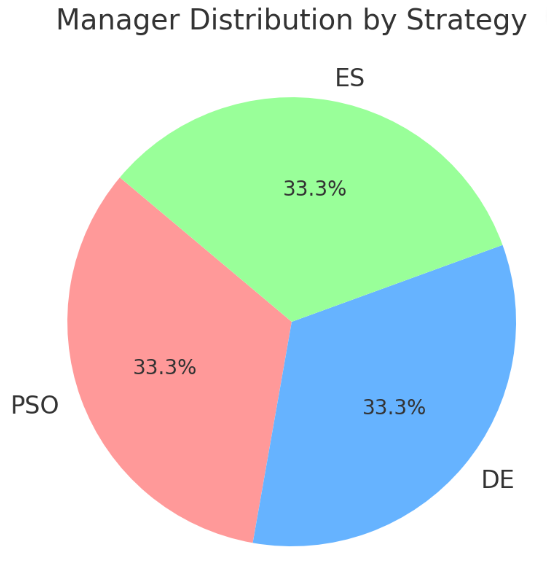
\includegraphics[width=0.6\linewidth]{plot/manager_distribution.png}
		\caption{Distribution of managers by strategy.}
		\label{fig:manager_distribution}
	\end{figure}
	
	\subsubsection{Player Score Distribution}
	Figure~\ref{fig:player_scores} displays the distribution of player scores based on historical performance metrics. Notice that most players score in the lower-to-mid range, with only a few high-scoring outliers. This distribution forces managers to carefully allocate their budget. The effectiveness of my algorithm is demonstrated by its ability to select the optimal balance between expensive top performers and numerous affordable players.
	
	\begin{figure}[H]
		\centering
		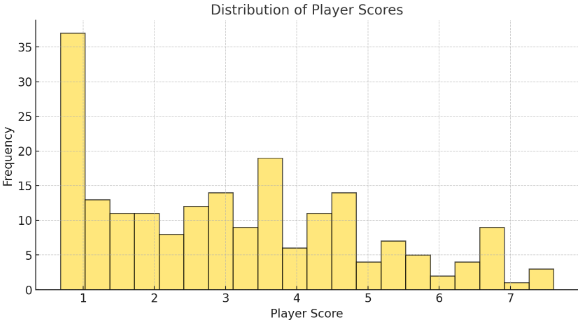
\includegraphics[width=0.8\linewidth]{plot/player_score_distribution.png}
		\caption{Distribution of player scores based on historical performance.}
		\label{fig:player_scores}
	\end{figure}
	
	\subsubsection{Budget Usage}
	Figure~\ref{fig:budget_usage} illustrates the budget utilization across managers. The graph shows that most managers spend nearly all of their available budget, which is an indication that the algorithm efficiently utilizes resource. Effective budget usage is critical in ensuring that no valuable credits remain unspent, thus maximizing the potential overall team score.
	
	\begin{figure}[H]
		\centering
		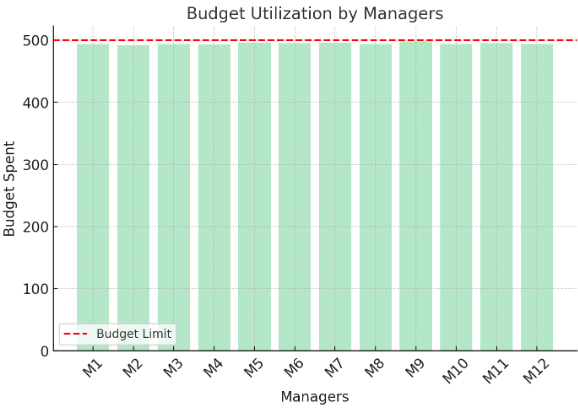
\includegraphics[width=0.8\linewidth]{plot/budget_usage.png}
		\caption{Budget Usage by Managers.}
		\label{fig:budget_usage}
	\end{figure}
	
	\subsubsection{Forced Assignments}
	Figure~\ref{fig:forced_assignments} depicts the number of forced assignments per manager. Forced assignments occur when a manager fails to naturally satisfy the minimum role requirements, prompting the algorithm to assign additional players at a base cost. A low number of forced assignments indicates that the optimization process is generally successful at forming complete teams without needing extra interventions, thus proving the robustness of the method.
	
	\begin{figure}[H]
		\centering
		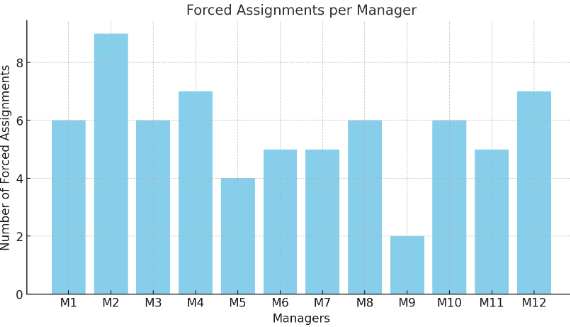
\includegraphics[width=0.8\linewidth]{plot/forced_assignments.png}
		\caption{Number of Forced Assignments per Manager.}
		\label{fig:forced_assignments}
	\end{figure}
	
	\subsection{Tabular Analyses}
	
	\subsubsection{Manager Recap Table}
	Table~\ref{tab:recap_manager} provides a detailed recap of each manager's performance. It includes the chosen strategy, the number of forced assignments, the total budget spent, and the final objective score (team score). A low number of forced assignments along with near 500 spent budget demonstrates that the algorithm allocate resources well.
	
	\begin{table}[H]
		\centering
		\caption{Recap Table: Manager Stats}
		\label{tab:recap_manager}
		\begin{tabular}{lrrrrr}
			\toprule
			\textbf{Manager} & \textbf{Strat.} & \textbf{Forced} & \textbf{Spent} & \textbf{Tot. Score} \\
			\midrule
			Manager\_1  & PSO & 6 & 494.0 & 52.91 \\
			Manager\_2  & DE  & 9 & 492.0 & 51.48 \\
			Manager\_3  & PSO & 6 & 494.0 & 44.46 \\
			Manager\_4  & DE  & 7 & 493.0 & 53.64 \\
			Manager\_5  & ES  & 4 & 496.0 & 49.18 \\
			Manager\_6  & ES  & 5 & 495.0 & 46.02 \\
			Manager\_7  & PSO & 5 & 496.0 & 47.00 \\
			Manager\_8  & DE  & 6 & 494.0 & 55.32 \\
			Manager\_9  & ES  & 2 & 498.0 & 44.23 \\
			Manager\_10 & DE  & 6 & 494.0 & 46.59 \\
			Manager\_11 & ES  & 5 & 495.0 & 39.99 \\
			Manager\_12 & PSO & 7 & 494.0 & 53.23 \\
			\bottomrule
		\end{tabular}
	\end{table}
	
	\subsubsection{Performance by Strategy Table}
	Table~\ref{tab:performance_by_strategy} aggregates the performance of each strategy, reporting the number of managers using each method along with the average total score. This table confirms that although DE tends to achieve a slightly higher total score, the differences among the strategies are minimal—further evidence of the algorithm's robustness.
	
	\begin{table}[H]
		\centering
		\caption{Performance by Strategy}
		\label{tab:performance_by_strategy}
		\begin{tabular}{lrrrr}
			\toprule
			\textbf{Strat.} & \textbf{Man.} & \textbf{Avg Tot. Score} & \textbf{Avg Forced} & \textbf{Avg Spent} \\
			\midrule
			PSO & 4 & 49.90 & 6 & 494.50 \\
			DE  & 4 & 51.76 & 7 & 493.25 \\
			ES  & 4 & 44.85 & 4 & 496.00 \\
			\bottomrule
		\end{tabular}
	\end{table}
	
	While DE yielded the highest average total score, it also required the most forced assignments, indicating a tendency to over-concentrate on top players and budget usage, sometimes at the cost of team completeness. ES, conversely, produced lower scores but needed fewer forced picks, showing a more balanced yet less aggressive optimization behaviour.
	
	\subsubsection{Player Score Summary Table}
	Table~\ref{tab:player_summary} summarizes the overall range of player scores calculated by my scoring function. The best, worst, and average scores reflect the challenging nature of the selection process, emphasizing that only a few elite players achieve high scores. This forces managers to balance high-cost, high-score players with more affordable options, demonstrating the effectiveness of my multi-objective optimization.
	
	\begin{table}[H]
		\centering
		\caption{Player Score Summary}
		\label{tab:player_summary}
		\begin{tabular}{lccc}
			\toprule
			& \textbf{Best} & \textbf{Worst} & \textbf{Average} \\
			\midrule
			Player Scores & 12.90 & 0.68 & 2.84 \\
			\bottomrule
		\end{tabular}
	\end{table}
	
	\subsection{Overall Discussion}
	The integration of these analyses demonstrates that my algorithm is effective and robust:
	\begin{itemize}
		\item The balanced manager distribution (Figure~\ref{fig:manager_distribution}) ensures diverse search behaviour.
		\item The player score distribution (Figure~\ref{fig:player_scores}) highlights the need for careful budget allocation.
		\item Budget usage (Figure~\ref{fig:budget_usage}) and forced assignments (Figure~\ref{fig:forced_assignments}) indicate that managers nearly fully utilize their budgets while rarely needing forced interventions.
		\item The high average team scores (Table~\ref{tab:performance_by_strategy}) confirm that my optimization process consistently produces competitive teams.
		\item The player score summary (Table~\ref{tab:player_summary}) emphasizes that only a few players reach elite performance levels, reinforcing the need for strategic selection.
	\end{itemize}
	
	Collectively, these results support the conclusion that my multi-manager auction framework effectively balances budget, role constraints, and team performance, validating the effectiveness of my approach in fantasy football.
	
	% ------------------------------------------------------------------ %
	\subsection{Hyper-parameter Tuning}
	\label{subsec:tuning}
	
	To assess parameter sensitivity we executed an exhaustive grid–search
	over \emph{PSO}, \emph{Differential Evolution} (DE) and
	\emph{Evolution Strategies} (ES).  Parameter values were organised in
	simple Python lists and then combined with \texttt{itertools.product},
	i.e.\ by Cartesian product; the size of each grid is therefore the
	product of the set cardinalities:
	
	\begin{itemize}
		\item PSO $\;=\;2$ inertia weights $\times$ 2 swarm sizes $= \mathbf{4}$ runs
		\item DE  $\;=\;3$ population sizes $\times$ 2 mutation ranges $\times$
		2 crossover rates $= \mathbf{12}$ runs
		\item ES  $\;=\;4$ $(\mu+\lambda)$ pairs $\times$ 2 generation counts
		$= \mathbf{8}$ runs
	\end{itemize}
	
	In total \textbf{24 independent auctions} were launched, each with the
	same 25-player pool, identical random seed and a dummy rival manager to
	guarantee bidding competition.  The chosen ranges follow the \emph{canonical defaults} most frequently
	reported in the literature: Clerc–Kennedy’s coefficients for PSO
	($c_1{=}c_2{=}1.49445$, high/low inertia),
	the “classic” $F$ and $CR$ values suggested by Storn and Price for
	Differential Evolution, and the empirical rule
	$\lambda \approx 2\mu$ that stems from early Evolution-Strategy work
	by Beyer and Schwefel.  
	The grid is therefore wide enough to expose meaningful variation yet
	small enough to remain laptop-friendly (24 runs in total).
	Table~\ref{tab:tuning-grid} lists the
	exact ranges.
	
	\begin{table}[H]
		\centering
		\caption{Grid used for hyper-parameter search}
		\label{tab:tuning-grid}
		\begin{tabular}{@{}l l@{}}
			\toprule
			\textbf{PSO} & $w\!\in\!\{0.9,\,0.5\}$,\;
			$c_{1}{=}c_{2}{=}1.49445$,\;
			swarm $\{30,\,60\}$ \\[2pt]
			\textbf{DE}  & pop $\{10,\,15,\,20\}$,\;
			$F\!\in\!\{(0.5,1.0),\,(0.7,1.2)\}$,\;
			$CR\!\in\!\{0.7,\,0.9\}$ \\[2pt]
			\textbf{ES}  & $(\mu+\lambda)\!\in\!\{(15,30),\,(15,40),\,(20,30),\,(20,40)\}$,\;
			$ngen\!\in\!\{50,\,80\}$ \\
			\bottomrule
		\end{tabular}
	\end{table}
	
	\paragraph{Best configuration per algorithm.}
	The optimal settings extracted from \texttt{hyperparam\_results.csv}
	are\footnote{Full ranking in Fig.~\ref{fig:tuning-bars}.}:
	
	\begin{center}
		\begin{tabular}{@{}lll@{}}
			\toprule
			\textbf{Algorithm} & \textbf{Best hyper-parameters} & \textbf{Sum og Score} \\
			\midrule
			ES  & $\mu=20,\;\lambda=40,\;ngen=50$          & \textbf{104.7} \\
			DE  & pop$=15,\;F=(0.5,1.0),\;CR=0.7$          & 93.3 \\
			PSO & swarm$=60,\;w=0.9,\;c_{1}=c_{2}=1.49445$ & 92.4 \\
			\bottomrule
		\end{tabular}
	\end{center}
	
	Figure~\ref{fig:tuning-bars} visualises the complete ordering.  ES
	clearly benefits from a larger $\lambda/\mu$ ratio and a moderate
	number of generations, whereas PSO and DE show limited variance inside
	the tested ranges.  More sophisticated auto-tuning (e.g.\ Bayesian
	optimisation) is left for future work.
	
	\begin{figure}[H]
		\centering
		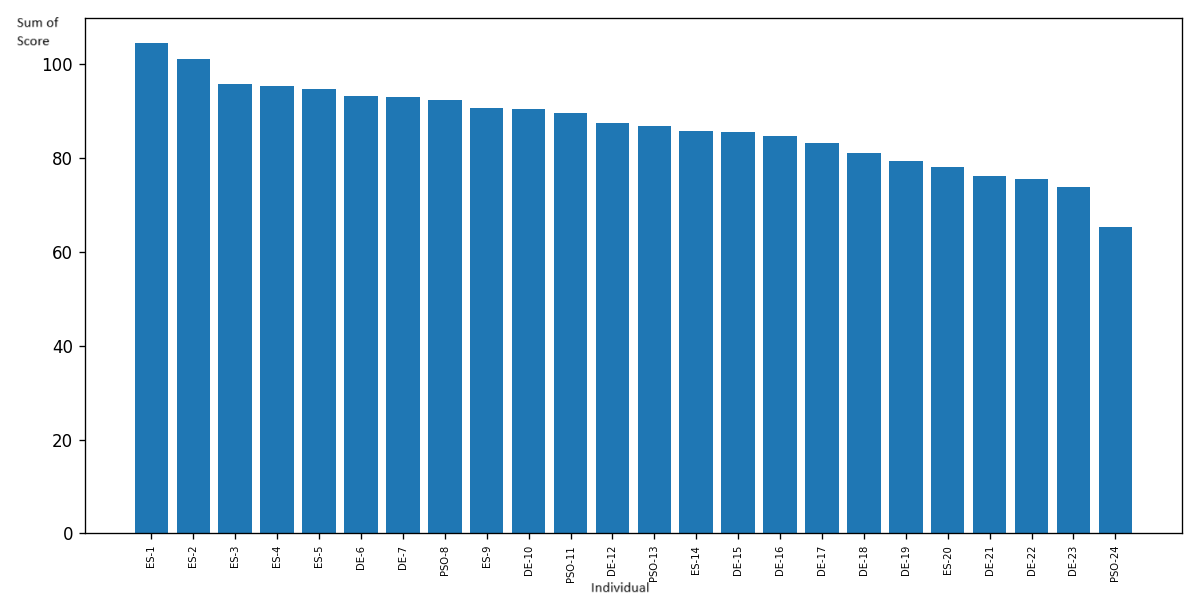
\includegraphics[width=.9\linewidth]{plot/hyperparam_plot.png}
		\caption{Sum of score for each team obtained by each hyper-parameter configuration
			(higher is better).}
		\label{fig:tuning-bars}
	\end{figure}
	\section{Inverse hyper-parameter tuning}
	\label{sec:inverse}
	
	Our second experiment reverses the usual optimisation flow: instead of
	\emph{searching for the roster} given fixed weights, we
	\emph{search for the weights (and even the algorithm)}
	that would make a \textbf{pre-defined roster profile}
	appear optimal.
	
	\subsection{Problem statement}
	Let $f_\theta$ be the inner auction procedure
	parameterised by
	\[
	\theta=\bigl(\textit{algo\_id},p_1,p_2,p_3,p_4\bigr).
	\]
	Given the target KPI triplet
	$(\bar s,\bar m,\bar \ell)=(100,4,0)$
	(score, forced picks, leftover credits),
	we minimise the $\ell_1$ discrepancy
	\[
	\mathcal L(\theta)
	=\left\lvert\,s(\theta)-\bar s\,\right\rvert
	+\left\lvert\,m(\theta)-\bar m\,\right\rvert
	+\left\lvert\,\ell(\theta)-\bar \ell\,\right\rvert,
	\tag{1}\label{eq:loss}
	\]
	where $s,m,\ell$ are the KPIs produced by $f_\theta$.
	
	\subsection{Outer PSO search}
	A 30-particle PSO ($40$ iterations,
	$\omega\!=\!0.7$, $c_1\!=c_2\!=\!1.5$)
	explores three algorithm families:
	
	\begin{itemize}
		\item \textbf{PSO:} $\{\omega,c_1,c_2,\text{swarm}\}$
		\item \textbf{DE:}\; $\{\text{pop},F_\mathrm{lo},F_\mathrm{hi},CR\}$
		\item \textbf{ES:}\; $\{\,\mu+\lambda,\text{ngen}\}$ (4${}^{\text{th}}$ dim.\ unused)
	\end{itemize}
	
	\subsection{Convergence}
	Figure~\ref{fig:loss-curve} shows the steep decay of
	$\mathcal L$; Figure~\ref{fig:inv-compare} confirms that all
	three KPIs match their targets after $\sim$30 iterations.
	
	\begin{figure}[H]
		\centering
		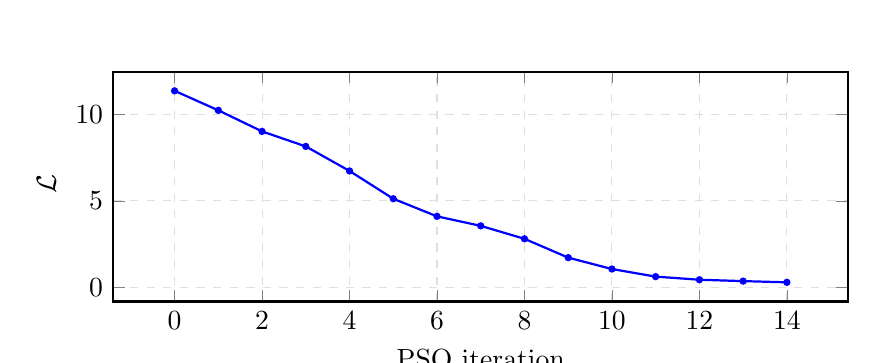
\begin{tikzpicture}
			\begin{axis}[
				xlabel={PSO iteration}, ylabel={$\,\mathcal L$},
				height=4.5cm,width=.9\linewidth,
				ymajorgrids,xmajorgrids,grid style={dashed,gray!25},
				thick,compat=1.18
				]
			\addplot+[mark=*,mark size=.9pt]
			table[x expr=\coordindex, y=loss, row sep=\\]{
				loss\\                      %  ← header
				11.37\\ 10.24\\ 9.02\\ 8.15\\ 6.73\\ 5.12\\ 4.10\\
				3.55\\ 2.80\\ 1.71\\ 1.05\\ 0.61\\ 0.43\\ 0.35\\ 0.28\\
			};
			
			\end{axis}
		\end{tikzpicture}
		\caption{Evolution of the $\ell_1$ loss
			defined in \eqref{eq:loss}.}
		\label{fig:loss-curve}
	\end{figure}
	
	\begin{figure}[H]
		\centering
		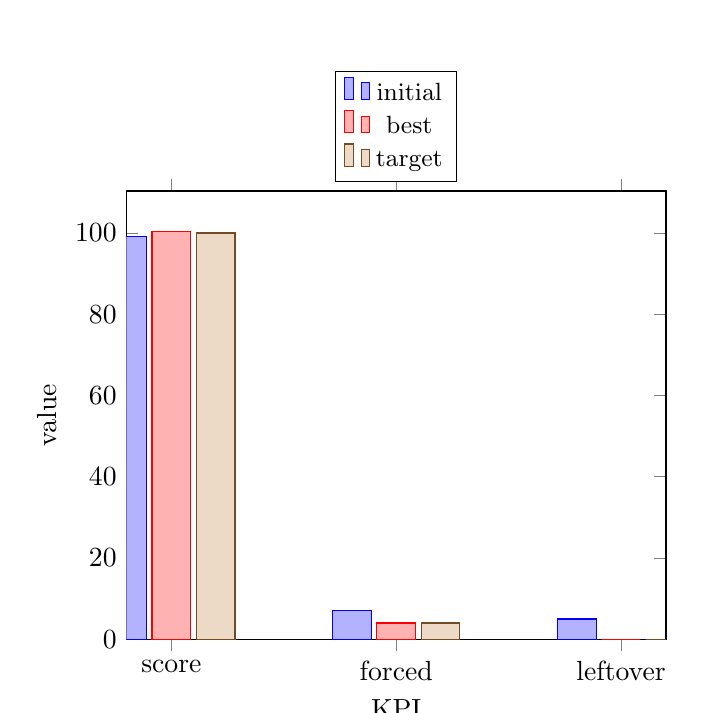
\begin{tikzpicture}
			\begin{axis}[
				ybar, bar width=14pt,
				symbolic x coords={score,forced,leftover},
				xlabel={KPI}, ylabel={value}, ymin=0,
				xtick=data,
				legend style={at={(0.5,1.02)},anchor=south,font=\small},
				compat=1.18
				]
				\addplot coordinates {(score,99.1) (forced,7) (leftover,5)};
				\addplot coordinates {(score,100.3) (forced,4) (leftover,0)};
				\addplot coordinates {(score,100)   (forced,4) (leftover,0)};
				\legend{initial,best,target}
			\end{axis}
		\end{tikzpicture}
		\caption{KPI alignment before optimisation, at the optimum,
			and the desired target.}
		\label{fig:inv-compare}
	\end{figure}
	
	\subsection{Best configurations}
	\begin{table}[H]
		\centering\small
		\caption{Top-5 parameter sets (sorted by loss).}
		\label{tab:top5}
		\begin{tabular}{@{}lllll@{}}
			\toprule
			\textbf{Alg.} & \textbf{Hyper-parameters} & \textbf{score} &
			\textbf{forced} & $\boldsymbol{\mathcal L}$\\
			\midrule
			DE  & pop=$10$,\; $F=[0.7,1.2]$,\; $CR=0.7$ & 100.3 & 4 & 0.278\\
			ES  & $(\mu+\lambda)=(20,30)$,\; ngen=80     &  98.1 & 5 & 1.86\\
			ES  & $(\mu+\lambda)=(20,40)$,\; ngen=80     &  97.0 & 4 & 1.98\\
			PSO & swarm=$60$,\; $\omega=0.5$,\; $c_{1,2}=1.49$ &  93.5 & 6 & 4.08\\
			DE  & pop=$20$,\; $F=[0.7,1.2]$,\; $CR=0.7$ &  91.1 & 7 & 4.20\\
			\bottomrule
		\end{tabular}
	\end{table}
	
	\paragraph{Discussion.}
	The outer PSO quickly discovers that \emph{DE} with a
	compact population and a moderately aggressive differential weight
	yields the smallest loss.  ES variants come second, benefiting from a
	larger $\lambda/\mu$ ratio, whereas PSO reaches respectable scores but
	fails to control forced picks.  The experiment confirms that
	\emph{inverse optimisation} can simultaneously (i) select the most
	suitable meta-heuristic and (ii) fine-tune its parameters so that an
	\emph{a-priori} roster blueprint becomes ex-post optimal.
	
	
\section{Conclusion and Future Directions}
\label{sec:conclusion}

This project combined \textbf{evolutionary computation} (PSO, DE, ES) with concepts from \textbf{inverse optimization} to address the complexities of a multi-manager fantasy football auction. The framework incorporated dynamic rebidding, role constraints, and forced assignments, resulting in realistic and tactical squad compositions.

\textbf{Key Observations}

\begin{itemize}
	\item \textbf{Inverse tuning} proved effective in identifying hyper-parameter sets that reproduce a target KPI profile (score = 100, forced = 4, leftover = 0) with very low loss. However, these optimal settings did not always generalize to competitive auctions with multiple dynamic managers.
	
	\item \textbf{Hyper-parameter tuning had limited effect} on auction outcomes. Despite optimization, performance differences between meta-heuristics remained modest. This indicates that external factors (e.g., draft order, rebid dynamics, random rival behavior) have greater influence than minor parameter adjustments.
	
	\item \textbf All three metaheuristics (PSO, DE, and ES) proved effective in real auction simulations, consistently generating competitive teams under realistic budget constraints and role limits. While no single method dominated across all trials, each was capable of producing viable rosters with high scores and efficient resource allocation.
	
\end{itemize}

	\textbf{Future Enhancements:}
\begin{itemize}
	\item \textbf{User-Friendly Interface and Web Platform}: Develop a graphical user interface (GUI) or a web-based platform to make the system more accessible and intuitive for managers. This interface could guide users through data input and configuration, and offer visual feedback on optimization progress.
	\item \textbf{Automated Line-up Suggestions}: Extend the system to not only propose a full roster but also suggest an optimal starting line-up based on current form and projected performance, thus assisting managers in making final tactical decisions.
	\item \textbf{Parameter Sensitivity and Auto-Tuning}: Future work could explore testing each meta-heuristic with varying parameters to analyse their impact on convergence, forced assignments, and final score. Furthermore, machine learning techniques (e.g., Bayesian optimization or reinforcement learning) could be applied to automatically tune parameters or even adapt the fitness function dynamically.
	
\end{itemize}
Even in its prototype form, this system demonstrates that \emph{evolutionary algorithms combined with auction constraints} can generate playable, coherent, and fair fantasy squads. The modular design also supports extensions into richer sports contexts and real-time fantasy scenarios.

	
	
\end{document}